\newpage
\subsubsection{UC2 - Addestramento del predittore}
\label{sssec:uc2}

\begin{figure}[h!]
  \begin{center}
    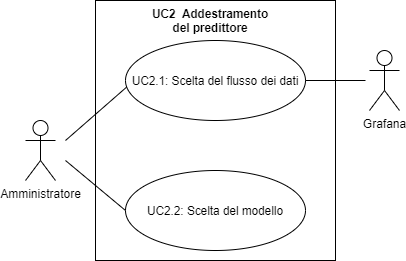
\includegraphics[width=19cm]{uc2.png}\\
    \caption{UC2 - Addestramento del predittore}%
    \label{fig:uc2}
  \end{center}
\end{figure}

\begin{itemize}
  \item \textbf{Attore primario}:  Utente;
  \item \textbf{Attore secondario}: Grafana;
  \item \textbf{Descrizione}: L'utente seleziona un flusso di dati presente in Grafana e il plug-in, grazie allo storico dei dati di quel flusso, addestra il predittore utilizzando un modello;
  \item \textbf{Precondizione}: L'utente ha creato un pannello del plug-in e sa che tipo di modello di machine learning va utilizzato;
  \item \textbf{Scenario principale}:
  \begin{enumerate}
    \item L'utente sceglie su che dati, tra quelli disponibili in Grafana, compiere l'addestramento (UC2.1);
    \item L'utente sceglie un modello da utlizzare per compiere l'addestramento(UC2.2).
  \end{enumerate}
  \item \textbf{Postcondizione}: Il plug-in ha generato il predittore ed ora è pronto a fare previsioni sui dati.
\end{itemize}

\paragraph{UC2.1 - Scelta del flusso dei dati}
\label{para:uc2.1}
\begin{itemize}
  \item \textbf{Attore primario}: Utente;
  \item \textbf{Attore secondario}: Grafana;
  \item \textbf{Descrizione}: L'utente sceglie su che flusso presente in Grafana compiere l'addestramento;
  \item \textbf{Precondizione}: L'utente ha a disposizione dei dati;
  \item \textbf{Scenario principale}: L'attore sceglie il flusso di dati per effettuare l'addestramento;
  \item \textbf{Postcondizione}: L'utente ha scelto un flusso di dati e con questo farà l'addestramento.
\end{itemize}

\paragraph{UC2.2 - Scelta del modello}
\label{para:uc2.2}
\begin{itemize}
  \item \textbf{Attore primario}: Utente;
  \item \textbf{Descrizione}: L'utente sceglie un modello da applicare ai dati tra SVM, RL, regressione esponenziale, regressione logaritmica, SVM adattata alla regressione o rete neurale;
  \item \textbf{Precondizione}:
  \item \begin{enumerate}
    \item L'utente ha scelto su che dati, tra quelli disponibili in Grafana, compiere l'addestramento (UC2.1);
    \item L'utente deve scegliere che modello di machine laerning utilizzare.
  \end{enumerate}
  \item \textbf{Scenario principale}: L'utente sceglie il modello da utilizzare per l'addestramento;
  \item \textbf{Postcondizione}: L'utente ha scelto il modello per l'addestramento;
  \item \textbf{Generalizzazioni}: UC2.2 viene generalizzato dai casi d'uso UC6, UC7, UC8, UC9, UC10 e UC11.
\end{itemize}

